\section{Utilizando o projeto}

Após a criação de um novo projeto podemos usar de duas formas: através de uma plataforma online com todas a ferramentas configuradas (codespaces). Ou configurando o projeto na máquina com o visual studio code.


\subsection{Utilizando de forma online com o Github Codespaces}

Para acessar o codespaces basta acessar a opção ``code > codespaces > create codespaces on main''. como na figura~\ref{fig:image04}

\begin{figure}[ht]
	\centering
	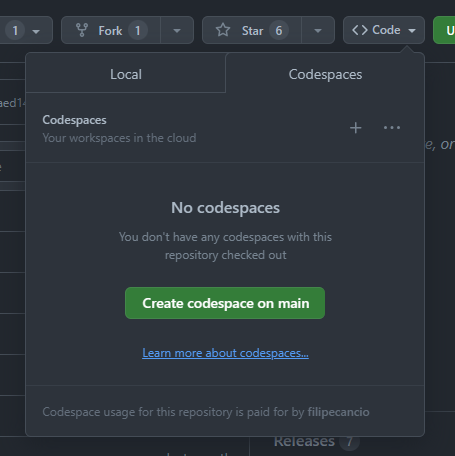
\includegraphics[width=.5\textwidth]{./images/image04.png}
	\caption{Criando um projeto novo no codespaces}
	\label{fig:image04}
\end{figure}

A partir daqui será redirecionada uma nova tela com uma versão online do Visual Studio Code com todo o projeto já configurado, pronto para ser usado.

\subsection{Utilizando de forma offline com o Visual Studio Code}

Para utilizar a versão offline é necessário ter instalado o git, MiKTeX o visual studio code e suas extensões (
LaTeX Workshop, latex-formatter, LaTeX LTeX,code runner). Após instalados basta fazer o clone do projeto e abrir no visual studio code.


A utilização do codespaces permite edição do projeto em qualquer dispositivo com internet, independente de suas especificações, porém usar o projeto na versão offline permite mais estabilidade no uso, visto que não é necessário o uso de internet.
Ao abrir o editor de texto escolhido haverá uma série de arquivos dispostos nas seguintes pastas:

- devcontainer: configuração padrão do projeto para rodar o LaTex de forma automática
- github: configuração de ações para criação de pdfs a cada versão do projeto.
- article: pasta contendo os arquivos Latex. Aqui faremos a edição do nosso texto adêmico.

Dentro da pasta ``article'' podemos encontrar:
- image: pasta com todas as imagens do.
- util: com os arquivos de configuração do LaTex. Nessa pasta é configurada as normas da SBC
- sections: fragmentos onde são escritos os artigos.
- main.tex: arquivo principal para produzir o texto acadêmico.

O Arquivo ``main.tex'' serve apenas para importar os arquivos presentes na pasta sections. Assim todo o texto deve ser produzido na pasta section, bastando em main,renomear arquivos modificados ou incluir novos artigos. Cada arquivo tex presente na pasta sections possui instruções produzidas pela própria SBC para a elaboração do texto acadêmico com LaTex.
A cada alteração e salvamento de algum arquivo no projeto, é gerado automáticamente um pdf com as mudanças feitas isso permite a visualização em tempo real da versão do projeto.
Abaixo podemos ver na imagem~\ref{fig:image05}, a exato momento da elaboração desse trecho do artigo pelo autor usando o codespaces uma visualização do pdf em tempo real.

\begin{figure}[ht]
	\centering
	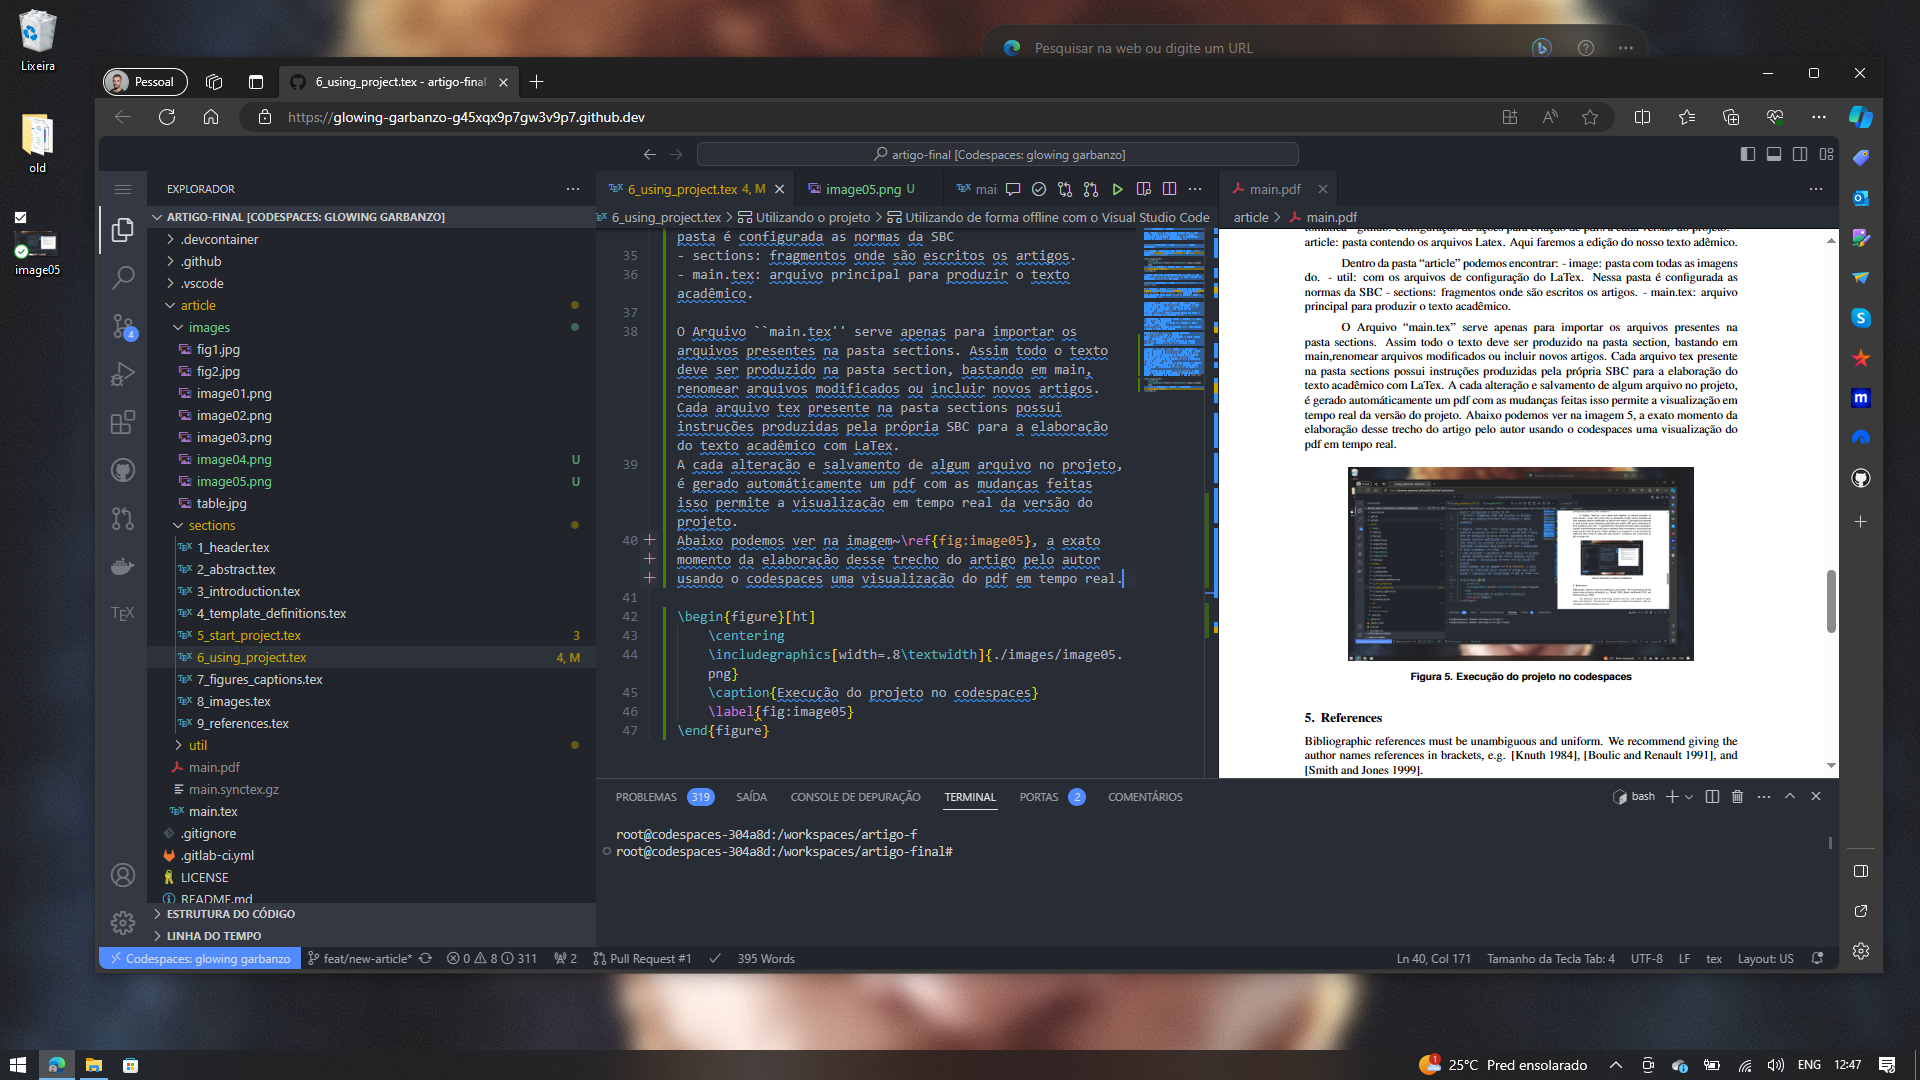
\includegraphics[width=.8\textwidth]{./images/image05.png}
	\caption{Execução do projeto no codespaces}
	\label{fig:image05}
\end{figure}